% file: problems/equal.tex

\section{DH Problem 5.9: $\equal(S_1, S_2)$}  \label{section:problem-5.9}
  Construct a function $\equal(S_1, S_2)$ that tests whether the strings $X$ and $Y$ are equal.
  It should return true or false accordingly.

  You may use the following operations:
  \begin{itemize}
    \item $\texttt{head}(X)$
    \item $\texttt{tail}(X)$
    \item $\texttt{last}(X)$
    \item $\texttt{all-but-last}(X)$
    \item $\texttt{eq}(s,t)$
  \end{itemize}
%%%%%%%%%%%%%%%%%%%%
\subsection{Solution}

The algorithm $\equal(S_1, S_2)$ is shown in Algorithm~\ref{alg:equal},
with appropriate assertions attached.

The partial correctness of $\equal$ can be denoted as
\marginnote{We are using the notations of Hoare logic developed by Tony Hoare.}

\begin{marginfigure}%
  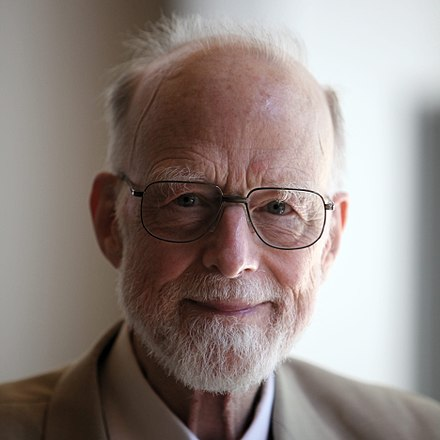
\includegraphics[width=0.60\linewidth]{figs/tony-hoare}
  \label{fig:hoare}
\end{marginfigure}

\marginnote{\cite{Hoare:CACM69}}

\[
  P \;\set{\equal}\; Q,
\]
meaning that if the input satisfies the precondition $P$
and the algorithm $\equal$ eventually terminates,
then the postcondition $Q$ must hold.
To this end, we show that:

% file: algs/equal.tex

\begin{algorithm}[t]
  \caption{Comparing two strings.}
  \label{alg:equal}
  \begin{algorithmic}[1]
    \Procedure{Equal}{$S_1,S_2$} 
      \LineComment{\teal{$P: S_1, S_2$ are strings}}
      \State $X \gets S_1$
      \State $Y \gets S_2$
      \State $E \gets \top$
      \hStatex

      \LineComment{\teal{(1) $I: S_1 = S_2 \iff X = Y \land E = \top$}}
      \While{$X \neq \epsilon \land Y \neq \epsilon \land E = \top$}
	\If{$\texttt{eq}(\texttt{head}(X), \texttt{head}(Y))$}
	  \State $X \gets \texttt{tail}(X)$
	  \State $Y \gets \texttt{tail}(Y)$
	\Else
	  \State $E \gets \bot$
	\EndIf
      \EndWhile

      \hStatex
      \LineComment{\teal{(2) $S_1 = S_2 \iff (X = \epsilon \land Y = \epsilon) \land E = \top$}}
      \If{$\lnot (X = \epsilon \land Y = \epsilon)$}
        \State $E \gets \bot$
	\LineComment{\teal{(3.1) $S_1 \neq S_2 \land E = \bot$}}
      \Else
	\State \texttt{DoNothing}  \Comment{Just for inserting an assertion here.}
	\LineComment{\teal{(3.2) $S_1 = S_2 \iff E = \top$}}
      \EndIf

      \hStatex
      \LineComment{\teal{(4) $Q: S_1 = S_2 \iff E = \top$}}
      \State \Return $E$
    \EndProcedure
  \end{algorithmic}
\end{algorithm}



\begin{enumerate}[(i)]
  \item $I$ is a loop invariant. That is,
    \[
      P \;\set{\texttt{Lines~\ref{line:init-begin}--\ref{line:init-end}}}\; I
    \]
    \[
      \big(I \land (X \neq \epsilon \land Y \neq \epsilon \land E = \top)\big) \;\set{\texttt{Lines~\ref{line:while-begin}--\ref{line:while-end}}}\; I
    \]
  \item $(2)$ is an invariant. It suffices to show that $(2)$ can be derived from
    \marginnote{This is a rather formal way. Be patient.}
    \renewcommand{\theequation}{\alph{equation}}
    \setcounter{equation}{0}
    \begin{gather}
      I \land \lnot (X \neq \epsilon \land Y \neq \epsilon \land E = \top) \nonumber\\
      = I \land (X = \epsilon \lor Y = \epsilon \lor E = \bot) \nonumber\\ 
      = \big(I \land (X = \epsilon)\big) \lor \big(I \land (Y = \epsilon)\big) \lor \big(I \land (E = \bot)\big) \label{eq:1st}
    \end{gather}
    in propositional logic by showing that each disjunct of (\ref{eq:1st}) implies $(2)$.

    Consider the first disjunct
    \renewcommand{\theequation}{\alph{equation}1}
    \setcounter{equation}{0}
    \begin{gather}
      I \land (X = \epsilon) \nonumber\\ 
      = (S_1 = S_2 \iff X = Y \land E = \top) \land (X = \epsilon)  \label{eq:1st-1st}
    \end{gather}
    It is required to prove both 
    \[
      \text{(\ref{eq:1st-1st})} \implies \Big(S_1 = S_2 \implies \big((X = \epsilon \land Y = \epsilon) \land E = \top \big)\Big)
    \]
    and 
    \[
      \text{(\ref{eq:1st-1st})} \implies \Big(\big((X = \epsilon \land Y = \epsilon) \land E = \top \big) \implies S_1 = S_2 \Big)
    \]
    \marginnote{Do you still remember how to prove an implication? What is the given? And what is the conclusion?
    Furthermore, when you derive $(2)$ from the third disjunct, 
    keep in mind that \emph{falsity implies everything}.}
    Now it is your (YES, it is YOU) job! It is also your job to deal with the second and the third disjuncts in a similar way.

    % \renewcommand{\theequation}{\alph{equation}3}
    % \setcounter{equation}{0}
    % \begin{gather}
    %   I \land (E = \bot) \nonumber\\ 
    %   = (S_1 = S_2 \iff X = Y \land E = \top) \land (E = \bot)  \label{eq:1st-3rd}
    % \end{gather}
  \item (3.1) is an invariant. It suffices to show that
    \[
      \big((2) \land \lnot (X = \epsilon \land Y = \epsilon) \land E = \bot\big) \implies (3.1).
    \]
    Stop reading! Take your pencil and paper! 
    \marginnote{\emph{Writing is nature’s way of letting you know how sloppy your thinking is.} \\ \hfill --- Richard Guindon (cartoon), 1989}
    Write down your arguments to convince yourself that the formula above indeed holds.
  \item (3.2) is an invariant. It suffices to show that
    \[
      \big((2) \land (X = \epsilon \land Y = \epsilon)\big) \implies (3.2).
    \]
    You already know how to prove this formula in propositional logic. Don't you?
    We now show you a more intuitive way to reason about programs:

    \marginnote{It proceeds \emph{semantically} rather than \emph{syntactically} as we have done before.}
    \emph{At point (2), we know that $S_1 = S_2$ if and only if $(X = \Lambda \land Y = \Lambda \land E = \top)$.
    At point (3.2), we further know that $(X = \Lambda \land Y = \Lambda)$. 
    Thus, at this point, we only need to check whether $E = \top$ to decide whether $S_1 = S_2$ holds.}
  \item $Q$ is an invariant. It suffices to show that
    \[
      \big((3.1) \implies Q\big) \land \big((3.2) \implies Q\big).
    \]
    It should be easy now for you to prove this formula.
\end{enumerate}
